\section{Physics-Infused ROM}

\begin{frame}
    \begin{center}
        \huge 2: \textbf{Formulation of PIROMs via Mori-Zwanzig Coarse Graining}
    \end{center}
\end{frame}

\begin{frame}{Formulation: Model-Order Reduction}
    \footnotesize
    \visible<1->{
    First step is \textbf{model-order reduction},}
    \begin{columns}
        \visible<2->{
        \begin{column}{0.35\textwidth}
            \begin{graybox}{Full-Order Model}
                \begin{align*}
                    \dot{\vx} &= \vF\left(\vx;\vp\right)\\
                    \vz_{\text{HF}} &= \vH\left(\vx;\vp\right)\\
                    \vx(t_0) &= \vx_0
                \end{align*}
                \vspace{-0.2in}
                \begin{enumerate}
                    \item<3-> $\vx\in\mathbb{R}^{n_x}$: states $(n_x\gg 1)$
                    \item<4-> $\vp\in\mathbb{R}^{n_p}$: parameters
                    \item<5-> $\vz_{\text{HF}}\in\mathbb{R}^{n_z}$: QoI 
                \end{enumerate}
            \end{graybox}
        \end{column}}
        \visible<6->{
        \begin{column}{0.65\textwidth}
            \begin{graybox}{Coarse Graining (reduce FOM's complexity)}
                \begin{enumerate}
                    \item<7-> State decomposition $\vx = \left[\bvx,\deltavx\right]^{\top}\in\mathbb{R}^{n_x}$ 
                    \begin{itemize}
                        \item<8-> Averaging variables (observables) $\bvx\in\mathbb{R}^{n_{\bar{x}}}$
                        \item<9-> Un-resolved (un-observables) $\deltavx\in\mathbb{R}^{n_{\delta x}}$ $\left(n_{\delta x}\gg n_{\bar{x}}\right)$
                    \end{itemize}
                    \item<10-> Projection operator $\cP:\cH_{n_x}\to\cH_{n_{\bar{x}}}\subset\cH_{n_x}$, e.g.,
                    \vspace*{-0.1in}
                    \begin{equation*}
                        \cP: \cG\left(\vx\right)\rightarrow \bar{\cG}\left(\bvx\right)\rightarrow\text{cheaper to evaluate!}
                        \vspace*{-0.1in}
                    \end{equation*}
                    \item<11-> Complement operator $\cQ = \cI - \cP$
                \end{enumerate}
                \vspace{-0.1in}
                \visible<12->{
                \begin{figure}
                    \centering
                    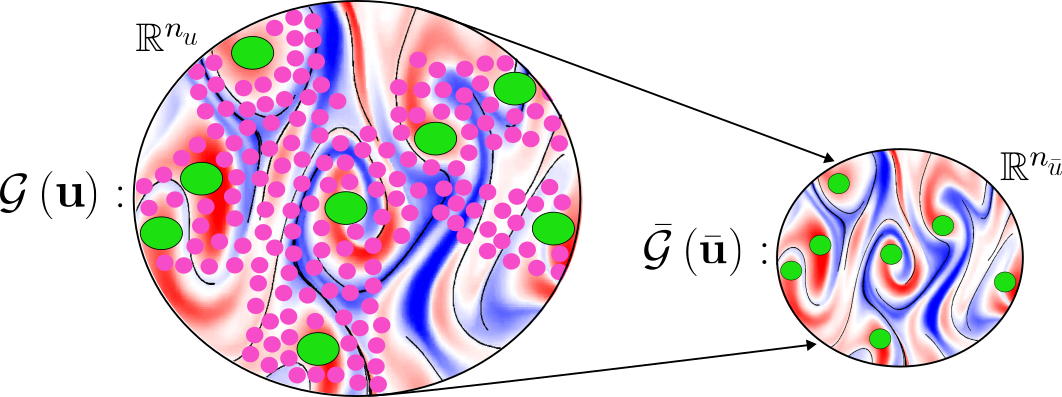
\includegraphics[width=0.7\textwidth]{../figs/pirom/coarse_graining.png}
                \end{figure}}
            \end{graybox}
        \end{column}}
    \end{columns}
\end{frame}

\begin{frame}{Formulation: Model-Order Reduction}
    \footnotesize
    \visible<1->{
    For example, define the projections $\vPhi\in\mathbb{R}^{n_x\times n_{\bar{x}}}$ and $\vPsi\in\mathbb{R}^{n_x\times n_{\delta_x}}$ such that [2],}
    \vspace*{-0.1in}
    \begin{columns}
        \begin{column}{0.55\textwidth}
            \visible<2->{
            \begin{graybox}{Coarse-Graining Dynamics}
                \begin{align*}
                    \visible<3->{
                    \bar{\vx} &= \vPhi^+\vx,\quad \vx = \vPhi\bar{\vx} + \vPsi\deltavx}\\
                    \visible<4->{
                    \dot{\vx} &= \vF\left(\vx;\vp\right)}\\
                    \visible<5->{
                    \frac{d}{dt}\left(\vPhi\bar{\vx} + \vPsi\deltavx\right) &= \vF\left(\vPhi\bar{\vx} + \vPsi\deltavx;\vp\right)}\\
                    \visible<6->{
                    \vPhi^+\frac{d}{dt}\left(\vPhi\bar{\vx} + \vPsi\deltavx\right) &= \vPhi^+\vF\left(\vPhi\bar{\vx} + \vPsi\deltavx;\vp\right)}\\
                    \visible<7->{
                    \dot{\bar{\vx}} &= \vPhi^+\vF\left(\vx;\vp\right)}\\
                    \visible<8->{
                    \dot{\bar{\vx}} &= \cP\left[\vPhi^+\vF(\vx;\vp)\right] + \cQ\left[\vPhi^+\vF(\vx;\vp)\right]}\\
                    \visible<9->{
                    &= \colorbox{green!30}{$\vr^{(1)}\left(\bvx,\vp\right)$} + \colorbox{red!30}{$\vr^{(2)}\left(\vx;\vp\right)$}}
                    \vspace*{-0.1in}
                \end{align*}}
                \centering
                \visible<2->{
                {\tiny $\vPhi^+$: left inverse of $\vPhi$, $\vPhi^+\vPsi = \vzero$}}
            \end{graybox}
        \end{column}
        \begin{column}{0.45\textwidth}
            \visible<10->{
            \begin{graybox}{Partitioned Dynamics}
                \centering
                \visible<11->{
                \begin{figure}
                    \centering
                    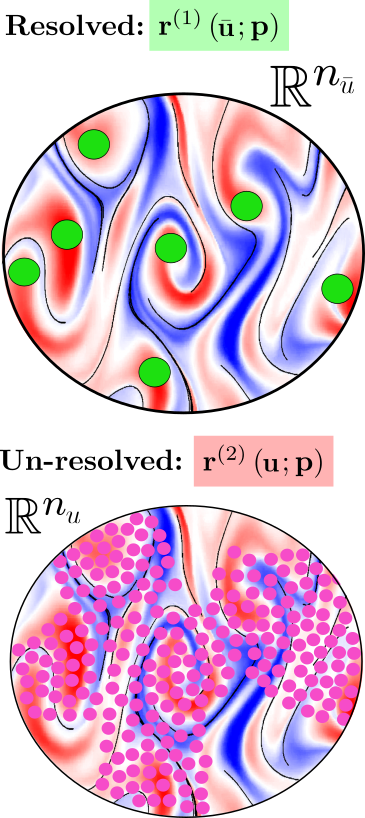
\includegraphics[width=0.42\textwidth]{../figs/pirom/partitioned_dynamics.png}
                \end{figure}}
                \vspace*{-0.1in}
                \visible<12->{
                {\tiny Need to \textbf{close} $\vr^{(2)}$ in terms of \textbf{resolved} variables only!}}
            \end{graybox}}
        \end{column}
    \end{columns}
\end{frame}

% \begin{frame}{Formulation: Model-Order Reduction}
%     \footnotesize
%     \visible<1->{
%     The FOM is effectively partitioned into \textbf{resolved} and \textbf{un-resolved} dynamics,
%     \begin{columns}
%         \begin{column}{0.5\textwidth}
%             \visible<2->{
%             \begin{graybox}{Resolved Dynamics}
%                 \begin{center}
%                     \colorbox{green!30}{$\dot{\bvx} = \vr^{(1)}\left(\bvx,t;\vp\right)$}
%                 \end{center}
%                 \vspace*{-0.1in}
%                 \begin{figure}
%                     \centering
%                     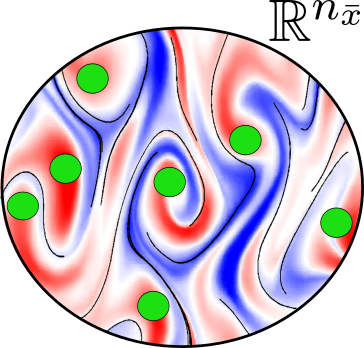
\includegraphics[width=0.6\textwidth]{../figs/pirom/resolved.png}
%                 \end{figure}
%             \end{graybox}}
%         \end{column}
%         \begin{column}{0.5\textwidth}
%             \visible<3->{
%             \begin{graybox}{Un-Resolved Dynamics}
%                 \begin{center}
%                     \colorbox{red!30}{$\dot{\bvx} = \vr^{(2)}\left(\vx,t;\vp\right)$}
%                 \end{center}
%                 \vspace*{-0.1in}
%                 \begin{figure}
%                     \centering
%                     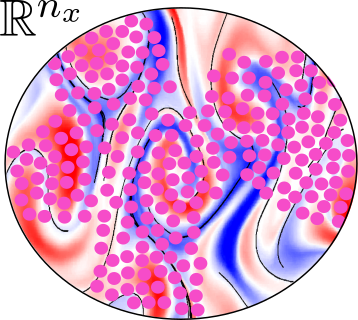
\includegraphics[width=0.6\textwidth]{../figs/pirom/unresolved.png}
%                 \end{figure}
%             \end{graybox}}
%         \end{column}
%     \end{columns}}
%     \begin{center}
%         \visible<3->{
%         However, need to \textbf{close} $\vr^{(2)}$ in terms of \textbf{resolved} variables only!}
%     \end{center}
% \end{frame}

\begin{frame}{Formulation: Physics-Infusion}
    \footnotesize
    \visible<1->{
    \textit{Mori-Zwanzig} helps in connecting \textbf{resolved} and \textbf{un-resolved} dynamics,}
    \visible<2->{
    \begin{equation*}
        \text{GLE}:\quad \underbrace{\frac{\partial}{\partial t} e^{t\cL}\bvx}_{\text{Observable Dynamics}} = \underbrace{e^{t\cL}\cP\cL\bvx}_{\text{Markovian}} + \underbrace{\int_0^t e^{(t-s)\cL}\cP\cL e^{s\cQ\cL}\cQ\cL\bvx ds}_{\text{Non-Markovian}} + \underbrace{e^{t\cQ\cL}\cQ\cL\bvx}_{\text{Noise}}
    \end{equation*}}
    \begin{columns}
        \visible<3->{
        \begin{column}{0.3\textwidth}
            \centering
            \textbf{Markovian}
            \begin{figure}
                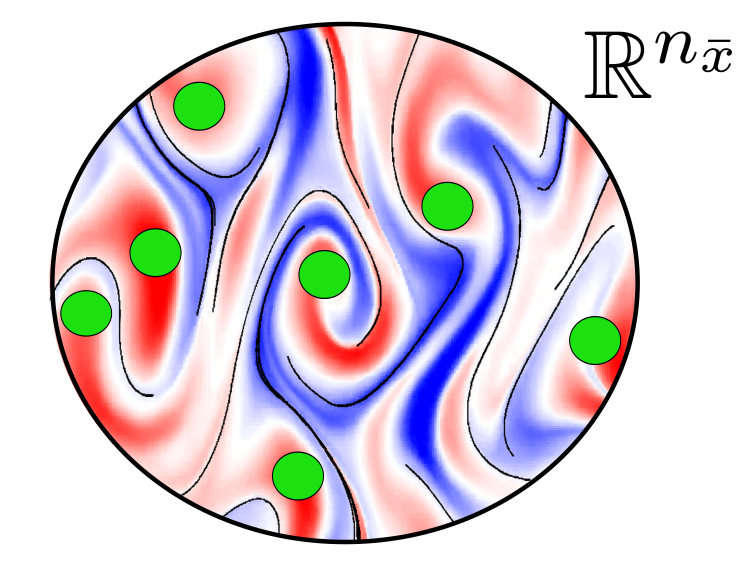
\includegraphics[width=0.9\textwidth]{../figs/pirom/coarse_variables.png}
            \end{figure}
            {\small (known dynamics)}
        \end{column}}
        \visible<4->{
        \begin{column}{0.3\textwidth}
            \centering
            \textbf{Non-Markovian}
            \begin{figure}
                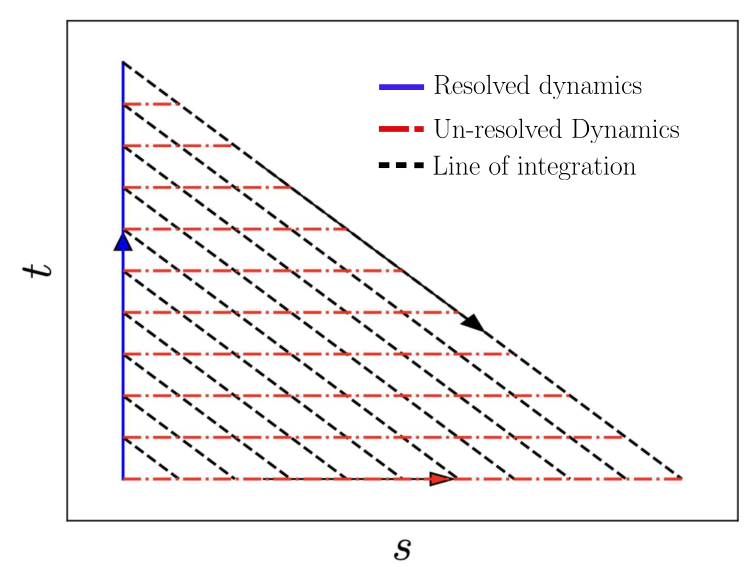
\includegraphics[width=0.9\textwidth]{../figs/pirom/memory.png}{\tiny [1]}
            \end{figure}
            {\small\textcolor{red}{(unknown dynamics)}}
        \end{column}}
        \visible<5->{
        \begin{column}{0.3\textwidth}
            \centering
            \textbf{Noise}
            \begin{figure}
                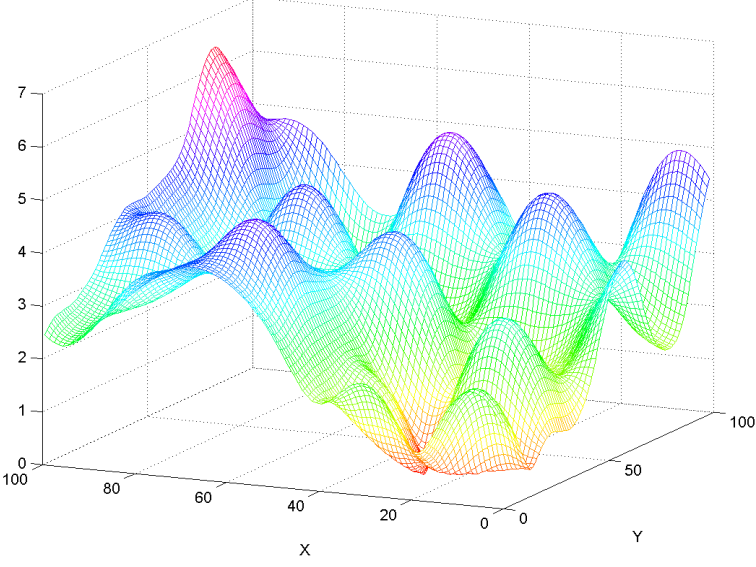
\includegraphics[width=0.9\textwidth]{../figs/pirom/noise.png}
            \end{figure}
            {\small\textcolor{black}{(orthogonal to $\cP$)}}
        \end{column}}
    \end{columns}
    {\tiny GLE: Generalized Langevin Equation, $\cL$: Liouville operator, PGEL: Projected GLE}
\end{frame}

\begin{frame}{Formulation: Physics Infusion}
    \footnotesize
    \begin{columns}
        \begin{column}{0.5\textwidth}
            \visible<1->{Applying the projection $\cP$ to the GLE,}
            \visible<2->{
            \begin{graybox}{Projected GLE (PGLE)}
                \visible<3->{
                \begin{equation*}
                    \frac{d\bvx}{dt} = \cP e^{t\cL}\cP\cL\bvx + \int_0^t \vkappa\left(\bvx,t,s;\vp\right)ds
                \end{equation*}}
                \vspace*{-0.1in}
                \begin{itemize}
                    \item<4-> $\cP e^{t\cL}\cP\cL\bvx$: coarse-grained \textbf{known} physics,
                    \item<5-> $\vkappa\left(\bvx,t,s;\vp\right)$: \textbf{unknown} memory kernel
                \end{itemize}
                \vspace*{-0.1in}
                \visible<6->{
                \begin{figure}
                    \centering
                    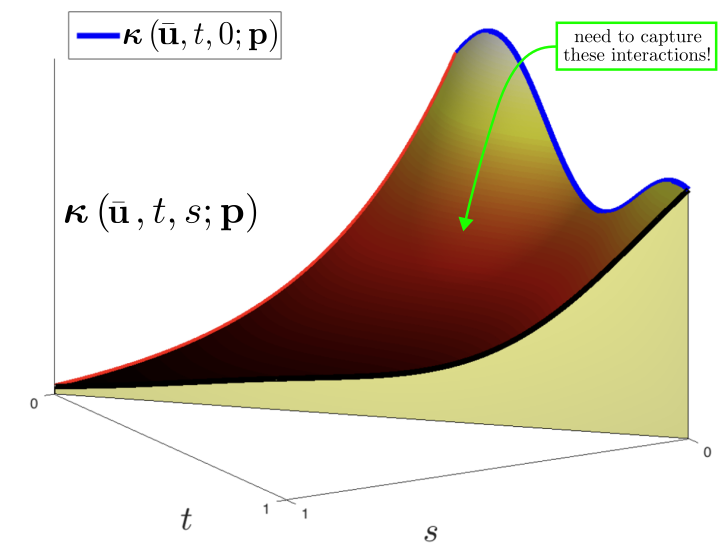
\includegraphics[width=0.6\textwidth]{../figs/pirom/memory_shape.png}{\tiny [1]}
                \end{figure}}
            \end{graybox}}
        \end{column}
        \begin{column}{0.5\textwidth}
            \visible<7->{
            \begin{graybox}{Memory Closure Examples}
                \begin{itemize}
                \item<8-> \textbf{Zeroth-Order Taylor Expansion:}
                \[\int_{0}^{t}\vkappa\left(\bvx,t,s;\vp\right) ds \approx t \vkappa\left(\bvx,t,0;\vp\right)\]
                \item<9-> \textbf{Parametric Ansatz:}
                \[\int_{0}^{t}\vkappa\left(\bvx,t,s;\vp\right) ds \approx \int_{0}^{t}\sum_{i=1}^{m}\boldsymbol{\theta}_i(\bvx,\vp)\phi_i(t,s)ds\]
            \end{itemize}
            \end{graybox}}
        \end{column}
    \end{columns}
\end{frame}

\begin{frame}{Formulation: Physics Infusion}
    \footnotesize
    \visible<1->{Adopt a \textbf{Markovian reformulation} to define a dynamical system parametrized by $\redvTheta\in\mathbb{R}^{n_{\Theta}}$,}
    \begin{columns}
        \begin{column}{0.5\textwidth}
            \visible<1->{
            \begin{graybox}{Kernel Approximation}
                \visible<2->{
                Parametrize the \textbf{memory kernel} as,}
                \visible<3->{
                \begin{equation*}
                    \vkappa(\bvx,t,s,\vp;\redvTheta) \approx \sum_{j=1}^{m} \cK_j(t,s,\bvx;\redvTheta)\phi_j(s,\bvx,\vp;\redvTheta)
                    \vspace*{-0.1in}
                \end{equation*}}
                \visible<4->{
                and \textbf{design} the $\ell$ and $\phi_j$ functions,}
                \visible<5->{
                \begin{align*}
                    \cK_j(t,s,\bvx;\redvTheta) &= e^{-\int_{s}^{t}\ell_j(\bvx,\tau;\redvTheta)d\tau}\Rightarrow\text{{\tiny \textbf{exponential decay!}}}\\
                    \phi_j(s,\bvx,\vp;\redvTheta) &= \text{{\tiny \textbf{informed structured!}}}
                \end{align*}}
                \vspace*{-0.1in}
            \end{graybox}}
        \end{column}
        \begin{column}{0.5\textwidth}
            \visible<6->{
            \begin{graybox}{Markovian Reformulation}
                \visible<7->{
                Define the \textbf{memory variables},}
                \visible<8->{
                \begin{equation*}
                    \beta_j(t) = \int_0^t \cK_j(t,s,\bvx;\redvTheta)\phi_j(s,\bvx,\vp;\redvTheta) ds
                \end{equation*}}
                \visible<9->{
                so that the \textbf{hidden dynamics} are,}
                \visible<10->{
                \begin{equation*}
                    \dot{\beta}_j = \phi_j(\bvx,\vp;\redvTheta) - \ell_j(\bvx,t;\redvTheta)\beta_j,\: j=1,\dots,m
                \end{equation*}}
                \visible<11->{
                Thus, \textbf{the PIROM may be written as},}
                \visible<12->{
                \begin{align*}
                    \dot{\bvx} &= \cP e^{t\cL}\cP\cL\bvx + \sum_{j=1}^{m}\beta_j\\
                    \dot{\beta}_j &= \phi_j(\bvx,\vp;\redvTheta) - \ell_j(\bvx,t;\redvTheta)\beta_j,\: j=1,\dots,m
                \end{align*}}
            \end{graybox}}
        \end{column}
    \end{columns}
\end{frame}

\begin{frame}{Formulation: Physics Infusion Overview}
    \footnotesize
    \begin{columns}
        \begin{column}{0.7\textwidth}
            \only<6>{
            \begin{figure}
                \centering
                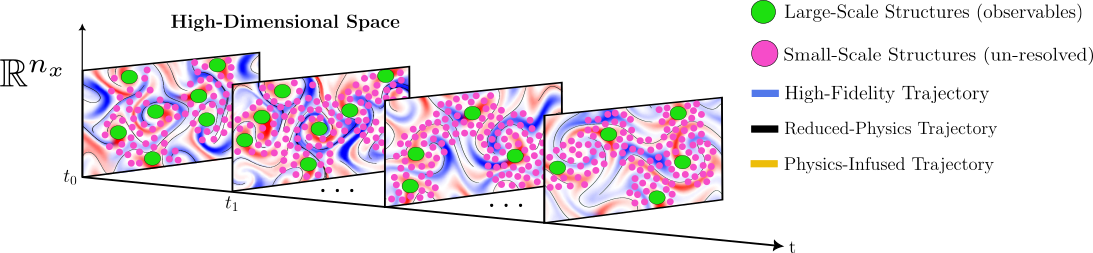
\includegraphics[width=0.9\textwidth]{../figs/pirom/pirom_overview_fom.png}
            \end{figure}}
            \only<7>{
                \begin{figure}
                    \centering
                    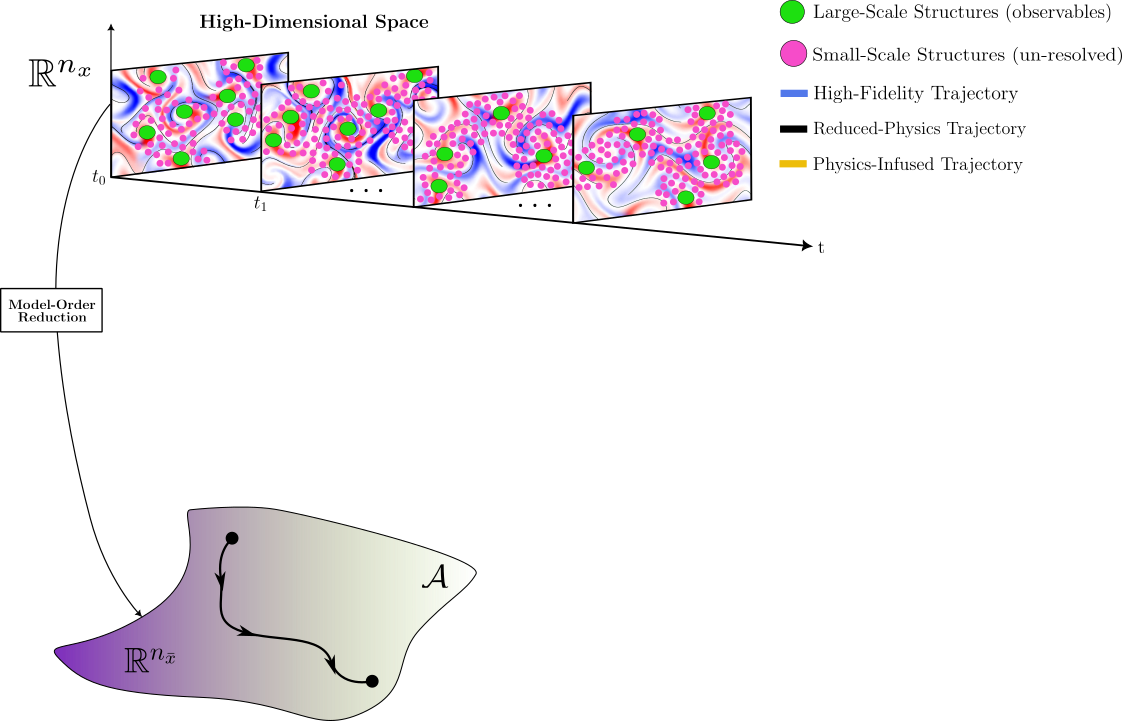
\includegraphics[width=0.9\textwidth]{../figs/pirom/pirom_overview_mor.png}
                \end{figure}}
            \only<8>{
                \begin{figure}
                    \centering
                    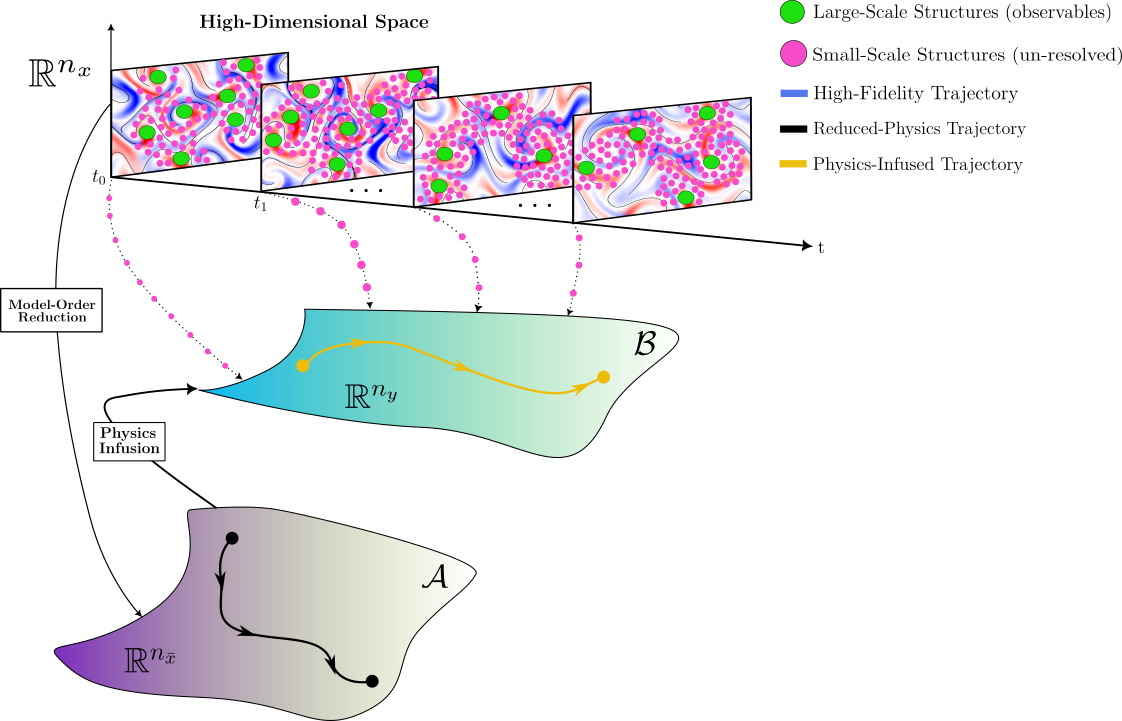
\includegraphics[width=0.9\textwidth]{../figs/pirom/pirom_overview_infusion.png}
                \end{figure}}
            \only<9->{
                \begin{figure}
                    \centering
                    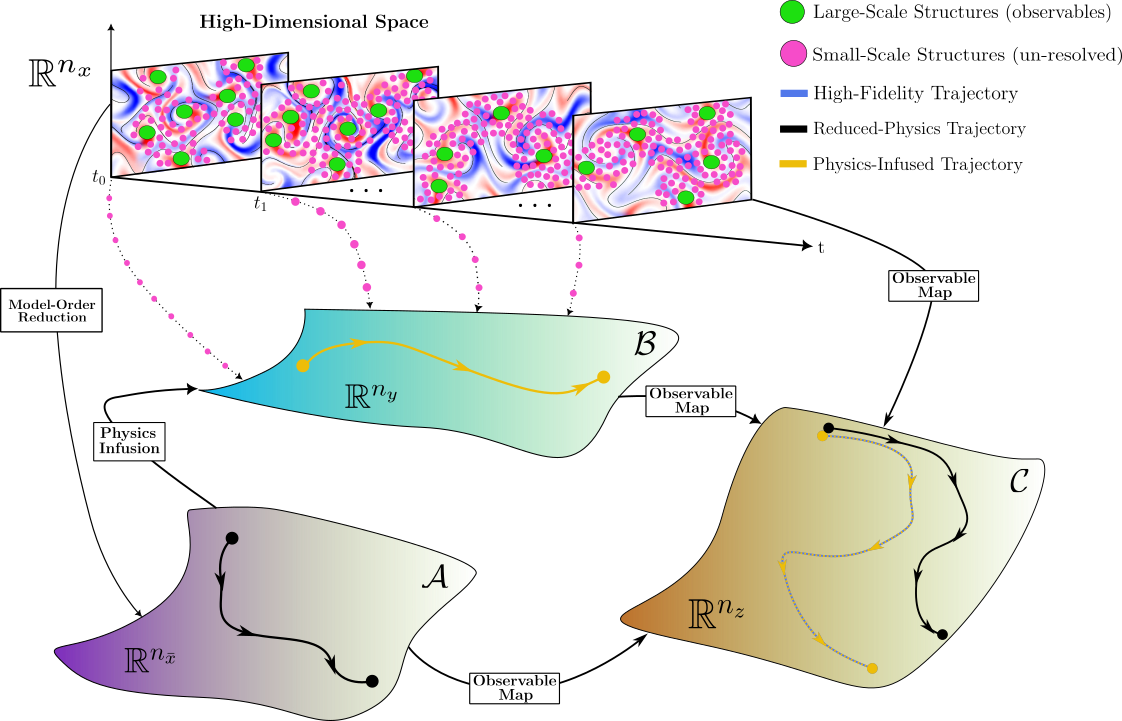
\includegraphics[width=0.9\textwidth]{../figs/pirom/pirom_overview.png}
                \end{figure}}
        \end{column}
        \begin{column}{0.3\textwidth}
            \centering
            \hspace{-0.1in}
            \footnotesize
            \visible<1->{
            \begin{graybox}{General Form of PIROM}
                \begin{align*}
                    \visible<2->{
                    \vy &= \underbrace{\left[\bvx,\vbeta\right]^\top}_{\text{PIROM states}}}\\
                    \visible<3->{
                    \boldsymbol{0} &= \underbrace{\boldsymbol{\mathcal{D}}\left(\vy,\dot{\vy},\vp;\redvTheta\right)}_{\text{physics-infused model}}}\\
                    \visible<4->{
                    \mathbf{c} &= \underbrace{\boldsymbol{\mathcal{G}}\left(\vy,\vp;\redvTheta\right)}_{\text{memory closure}}}\\
                    \visible<5->{
                    \vz &= \underbrace{\boldsymbol{\mathcal{H}}\left(\vy,\vp;\redvTheta\right)}_{\text{observable map}}}\\
                    \visible<6->{
                    \boldsymbol{0} &= \underbrace{\vPsi_0\left(\vy(t_0),t_0;\redvTheta\right)}_{\text{initial condition}}}
                \end{align*}
            \end{graybox}}
            \visible<10->{
            {\footnotesize \textcolor{red}{The parameters $\vTheta$ are learned from data!}}}
        \end{column}
    \end{columns}
\end{frame}

